\chapter{Pruebas}

	\noindent En este capítulo se presentará una breve descripción acerca de las distintas pruebas realizadas, los resultados obtenidas en casa una de ellas, así como el procedimiento que se siguio.
	Se mencionarán distintos tipos de pruebas realizadas con la finalidad de omitir lo más posible los errores que puedan presentarse siendo usada por los usuarios finales. \\
	
	\section{Plan de pruebas}
	\noindent La finalidad de realizar pruebas antes de que el proyecto sea entregado al usuario final es mitigar en su mayoría o totalidad los posibles errores que puedan presentarse, de tal manera que, para el equipo de desarrollo se le informa de errores que pudieron omitirse durante el análisis del mismo y a su vez proporciona confianza al cliente en cuanto al funcionamiento del proyecto.
	
	\noindent Por tal motivo se llegó a la conclusión de realizar pruebas al proyecto propuesto para identificar posibles errores que no se contemplaron en el análisis del mismo y lo más importante, proporcionarle al usuario final una aplicación web que no tenga fallos constantes. 
	
	\noindent Las primeras pruebas que se realizaron fueron las pruebas unitarias, las cuales consistieron en realizar pruebas sencillas de tal manera que se comprobara que al hacer uso de cada módulo desarrollado no tuviese errores.\\
	Mencionando algunas de las pruebas fue el verificar que en las entradas de un formulario no presentará errores, se comprobó que existiesen los mensajes y validaciones previamente definidas.
	
	\noindent Posteriormente se realizaron pruebas de sistema, estas consisten en ir agregando de manera progresiva los módulos desarrollados y, que cumpliesen con las pruebas unitarias. De tal manera, se verifica que la conexión entre distintas vistas o módulos tuvieran un buen resultando tomando en cuenta los mensajes y validaciones previamente definidos. \\
	
	\noindent Una vez que se concluyeron las pruebas de sistema nos acercamos con alumnos de la Escuela Superior de Cómputo para informarles en primer instancia, el funcionamiento del proyecto, a quién va dirigido y algunos puntos relevantes del desarrollo del mismo con lo antes mencionado se obtuvo lo siguiente:
	
	\begin{figure}[hbt!]
		\centering
		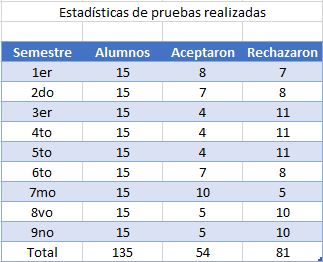
\includegraphics[width=8cm, height=8cm]{Imagenes/tablaEstadisticas}
		\caption{Tabla del número de alumnos considerados para las pruebas.}
		\label{tablaestadisticas}
	\end{figure}

	\begin{figure}[hbt!]
		\centering
		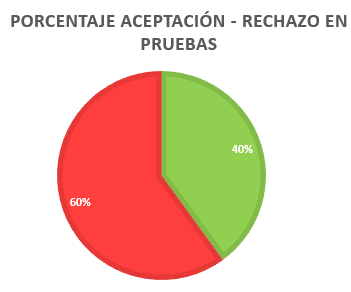
\includegraphics[width=8cm, height=6cm]{Imagenes/graficaEstadisticas}
		\caption{Gráfica corresponidente a la Tabla de alumnos considerados para las pruebas.}
		\label{graficaestadisticas}
	\end{figure}
	
	\noindent Considerando los resultados obtenidos, se recabó información de errores que no se habían contemplado. Otro punto importante fue el porcentaje de alumons que se negaron a participar en la prueba del proyecto sin embargo, con los datos obtenido se logró obtener una mejora en el proyecto. 
	
	\noindent No obstante, para complementar la etapa de pruebas del proyecto nos basamos en las pruebas Clases de Equivalencia. En la cual se se plantean los posibles casos que se pueden llegar a presentar en un módulo. Estos casos se crean o toman con base en el caso de uso correspondiente, es decir, por cada caso de uso que se tiene en el sistema debe existir un guión de prueba.\\
	
	\noindent La ventaja con este tipo de pruebas es que nos permite cubrir todos los posibles escenarios en un módulo en específico. Para saber el número de pruebas que son necesarias realizar se debe seguir la siguiente formula matemática:\\
	$ n1 * n2 * ... * n_{n} $ \\
	donde, 
	n, corresponde al número de entradas que tiene el caso de uso.\\
	n1, este valor corresponde al número de pruebas que se realicen en cada uno de las entradas del caso de uso.\\
	
	\noindent Ahora bien, hay otra formula la cual indica el número de pruebas minímas necesarías para considerar que el caso de uso analizando tiene cálidad, la formula matemática es la siguiente: \\
	
	$ (n1 + n2 + ... + n_{n}) - (n - 1) $
	
	n, corresponde al número de entradas que tiene el caso de uso.\\
	n1, este valor corresponde al número de pruebas que se realicen en cada uno de las entradas del caso de uso.\\
	
	\noindent Tomando en cuenta lo antes mencionado, se realizaron las pruebas correspondientes, a continuación se mostrarán los guiónes de prueba de alguno de los módulos representativos de la aplicación web.\\
	\pagebreak
	
	\textbf{Guión de prueba del caso de uso 10: Agrega resultados}
	
	\begin{figure}[hbt!]
		\centering
		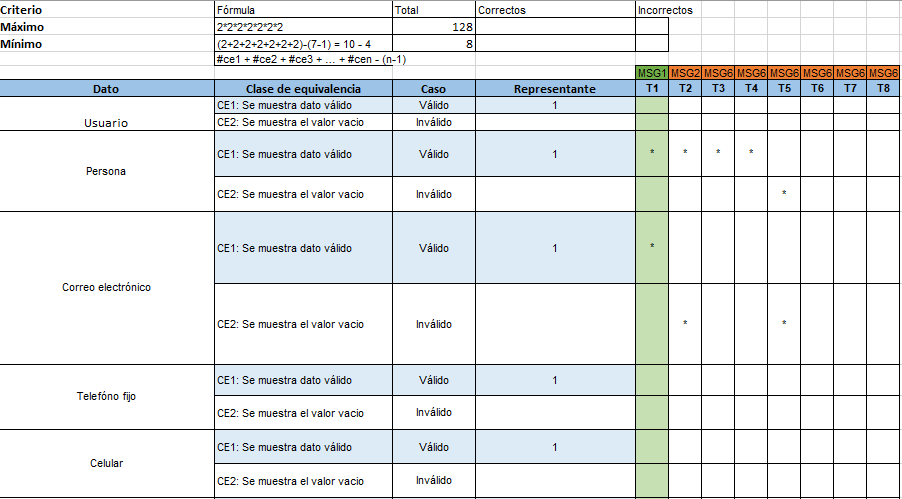
\includegraphics[width=14cm, height=6cm]{Imagenes/Pruebas/GuionPruebaCU10}
		\caption{Tabla correspondiente al guión de prueba del caso de uso 10}
		\label{guionpruebaCU10}
	\end{figure}

	\textbf{Guión de prueba del caso de uso 11: Agrega resultados}

	\begin{figure}[hbt!]
		\centering
		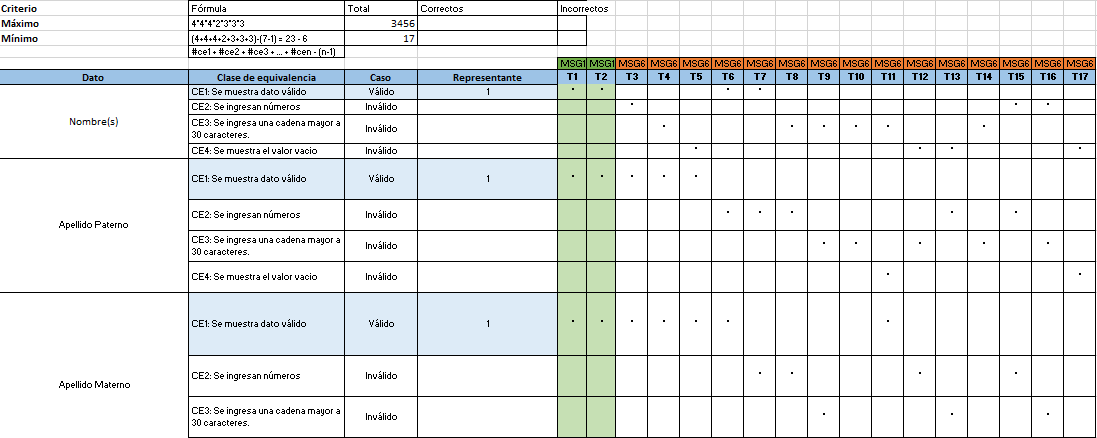
\includegraphics[width=14cm, height=6cm]{Imagenes/Pruebas/GuionPruebaCU11}
		\caption{Tabla correspondiente al guión correspondiente al CU11}
		\label{guionpruebaCU11}
	\end{figure}
\pagebreak

	\textbf{Guión de prueba del caso de uso 11: Agrega resultados}
	\begin{figure}[hbt!]
		\centering
		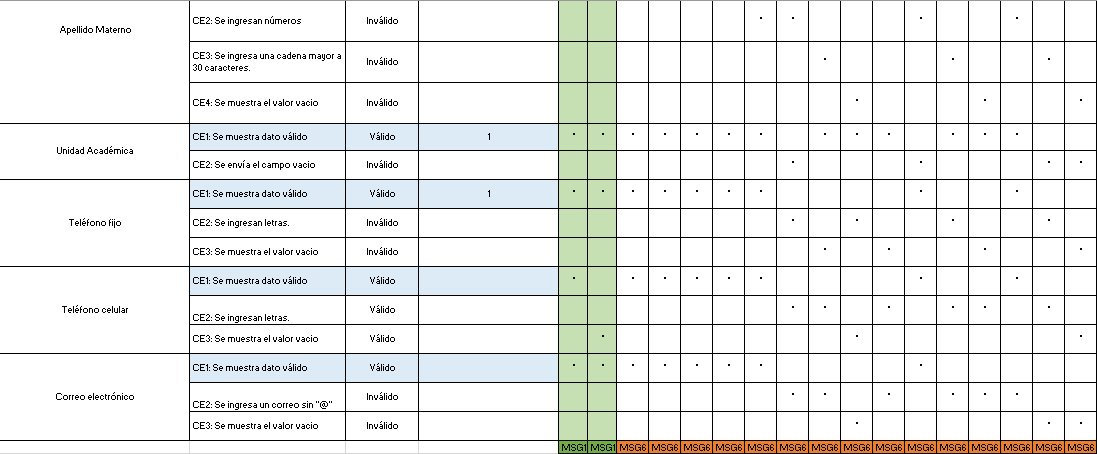
\includegraphics[width=14cm, height=6cm]{Imagenes/Pruebas/GuionPruebaCU11_1}
		\caption{Tabla correspondiente al guión correspondiente al CU11}
		\label{guionpruebaCU11_1}
	\end{figure}

	\textbf{Guión de prueba del caso de uso 15: Agrega resultados}
	\begin{figure}[hbt!]
		\centering
		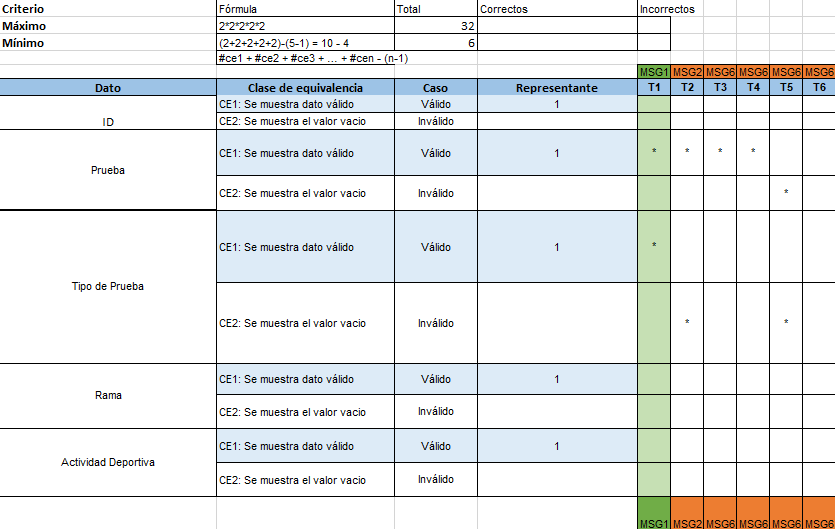
\includegraphics[width=14cm, height=6cm]{Imagenes/Pruebas/GuionPruebaCU15}
		\caption{Tabla correspondiente al guión correspondiente al CU15}
		\label{guionpruebaCU15}
	\end{figure}
\pagebreak
	
	\textbf{Guión de prueba del caso de uso 16: Agrega resultados}	
	\begin{figure}[hbt!]
		\centering
		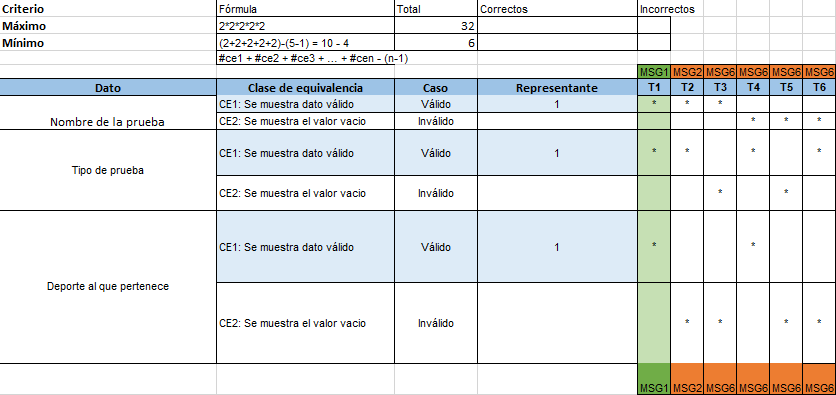
\includegraphics[width=14cm, height=6cm]{Imagenes/Pruebas/GuionPruebaCU16}
		\caption{Tabla correspondiente al guión correspondiente al CU16}
		\label{guionpruebaCU16}
	\end{figure}
	
	\textbf{Guión de prueba del caso de uso 22: Agrega resultados}	
	\begin{figure}[hbt!]
		\centering
		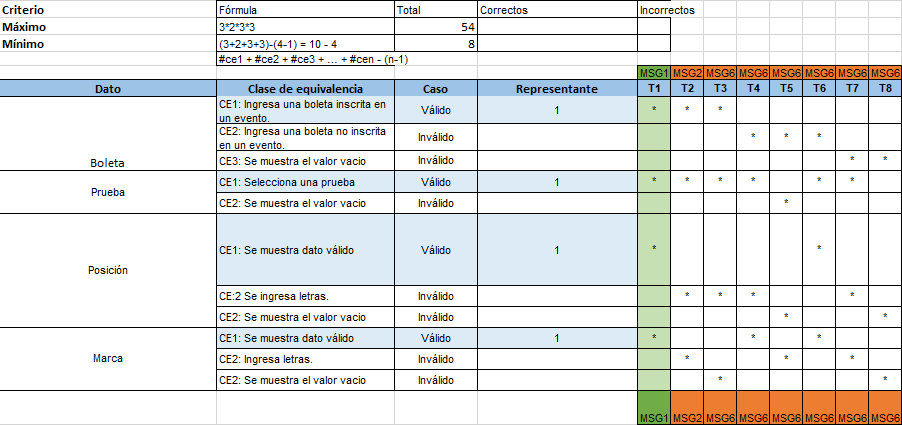
\includegraphics[width=14cm, height=6cm]{Imagenes/Pruebas/GuionPruebaCU22}
		\caption{Tabla correspondiente al guión correspondiente al CU22}
		\label{guionpruebaCU22}
	\end{figure}
	
	
	